%-----------------------------------------------------------------
% POSTER CONTENTS
% !TEX root = ../main.tex
%-----------------------------------------------------------------

\begin{block}{Introduction}
	% \nocite{Webster2005}
	\nocite{Hinkley1997}
	% \nocite{Osso2009}
	For the North Atlantic (N.~Atl.) basin, it has been shown \cite{Corral2010} that the probability distribution of the so-called power-dissipation index ($PDI$, a rough estimation of released energy) is indeed affected by the annual and basin-wide averaged sea surface temperature (SST), displacing towards more extreme values on warm years (high-SST).
	As the $PDI$ integrates (cubic) wind speed over tropical-cyclone (TC) lifetime, it is an open question where the $PDI$ increase comes from (higher speed, longer lifetime, or both).
\end{block}

\begin{block}{Data}
	To characterise a TC one needs to define a physically relevant measure of released energy. The released energy of each TC is summarised as
	\begin{equation}\label{eq:pdi}
		PDI = \sum_{t} v_{t}^{3} \Delta t .
	\end{equation}
	The raw hurricane best track data (HURDAT2) is provided by the National Hurricane Center. We intentionally limit this study to the satellite era (1966--2016), as it is the most reliable.

	\bigskip
	Then, the hurricane observational data is classified into occurrences in low-SST and high-SST years depending on whether they are lower or greater than
	\begin{equation}
		\ev{\text{SST}} = \sum_{y \in Y} \frac{\text{SST}(y)}{Y} ,
	\end{equation}
	where $\text{SST}(y)$ is the mean SST of the year $y$, and $Y$ is the total number of years studied. The SST data (HadISST1) is provided by the Met Office Hadley Centre.

\end{block}

\begin{block}{ }
	\begin{figure}
		\vspace*{-1.1cm}
		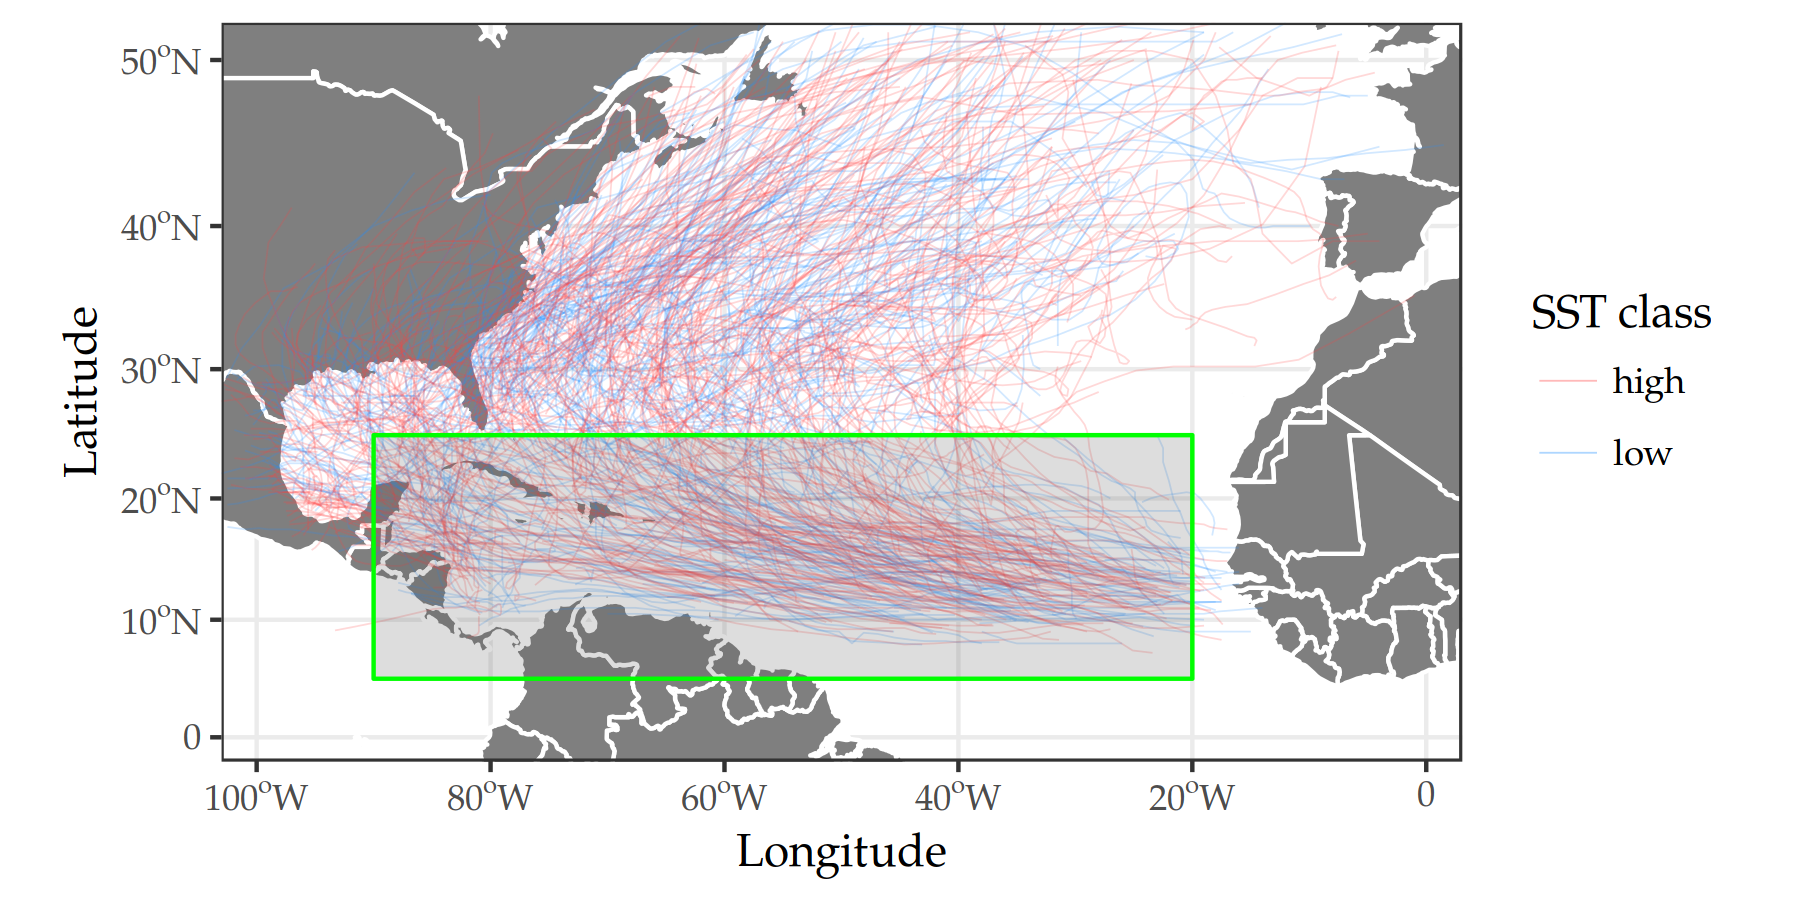
\includegraphics[width=0.84\linewidth]{images/natl_map.png}
		\caption{~Tropical-cyclones best tracks for the North Atlantic basin}
	\end{figure}
\end{block}

%-----------------------------------------------------------------
\begin{block}{Hypothesis}
	%\begin{multicols}{2}
	The hypothesis is that the $\text{SST}$ does not directly affect the maximum wind speed of a TC: storms of equal duration should, in theory, have the same wind speed and $PDI$, and have the same joint distribution:
	\begin{equation}
		f(Y \mid X = x)_{\text{low}} = f(Y \mid X = x)_{\text{high}} .
	\end{equation}
	The physical reasoning behind this is that once the cyclone is activated, the wind speed should not depend on its underlying $\text{SST}$.
	%\end{multicols}
% \end{block}

% %-----------------------------------------------------------------
% \begin{block}{Methodology}
	%\begin{multicols}{2}
	Instead of working with the exact joint
	%bivariate log-normal
	distributions $f$, we study the expected value of the distributions:
	\begin{equation}
		E(Y \mid X = x )_{\text{low}} = E(Y \mid X = x )_{\text{high}},
	\end{equation}
	where $E(Y \mid X = x )$ is estimated by performing a ordinary least squares (OLS) regression analysis on the data sets.

	% \medskip
	% It is important to notice that the relationships between the TC variables are of non-linear nature. This naturally means that our regressions need to follow a so-called log--log model:
	% \begin{equation}\label{eq:lm-model-bis}
	% 	\log \Psi = \alpha + \beta \log \Phi + \epsilon ,
	% \end{equation}
	% where $\log \Psi \equiv Y$ and $\log \Phi \equiv X$.
	% \medskip
	%\end{multicols}
\end{block}

% \vspace*{-1cm}
% \begin{block}{}
% 	%\begin{multicols}{2}
% 	In essence, our methodology will consist in comparing the low-SST and high-SST regression models using non-parametric permutation tests.

% 	\medskip
% 	For the permutation tests, we use bootstrap %and
% 	\nocite{Analysis2003} %the bootstrap-$t$ method
% 	in order to get a better estimation of the value of the different studied statistical coefficients (such as $\hat{\alpha}$, $\hat{\beta}$, $r^{2}$) and their standard errors than the one obtained using the value obtained using the OLS method. Withal, we compare the results obtained using both methods.

% 	% We compare the results obtained using (a) the OLS method, and (b) the bootstrap-$t$ method
% 	%\end{multicols}
% \end{block}

\begin{block}{Data shows}
	Our empirical results show a remarkable correlation in the joint distribution of lifetime and wind speed, as seen in \Cref{fig:regression}. The marginal distributions can be seen in \Cref{fig:natl-marginals}.

	\begin{figure}
		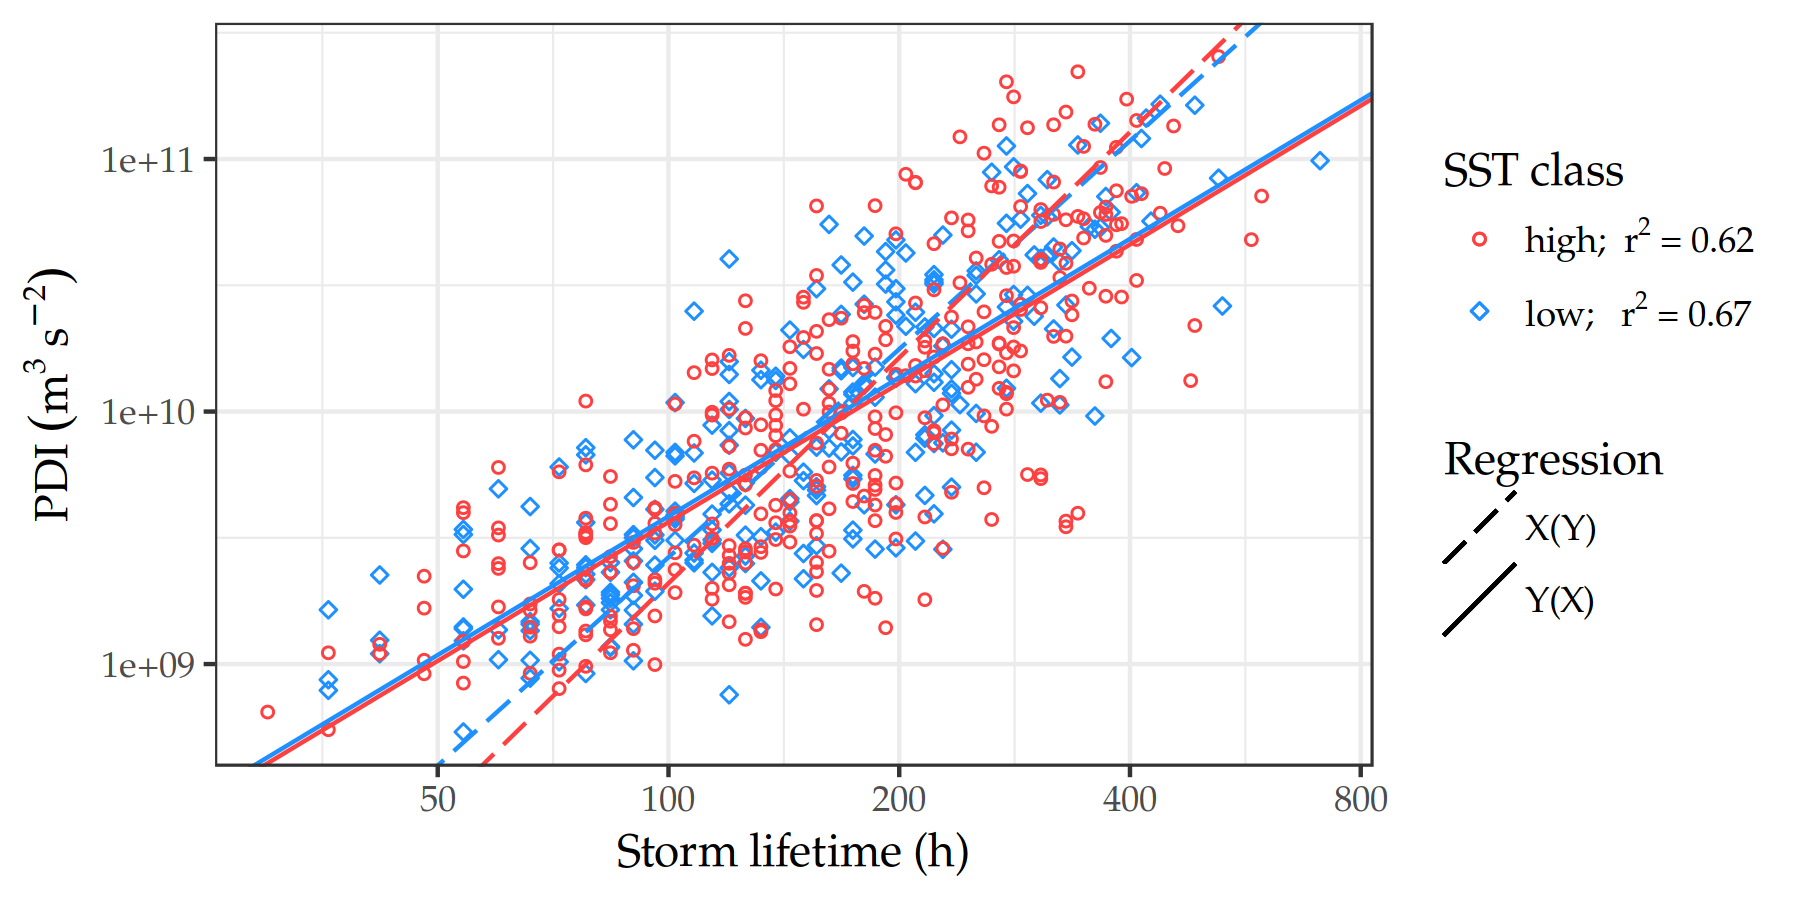
\includegraphics[width=0.84\linewidth]{images/scatter_natl.png}
		\caption{~$PDI$ vs lifetime regression analysis for tropical-cyclones (excluding tropical depressions) on the North Atlantic basin}
		\label{fig:regression}
	\end{figure}
\end{block}
